\chapter{Tuning \& Optimisation}
After we build a basic structure of our project, we noticed that several issues can be refined and improved.

\section{Mathematical Morphology}\label{sec:MM}
We use mathematical morphology to reduce efficiently calculation by increasing the number of 0s in image matrix and keeping original character structures to maximum extent simultaneously. And images loaded from disk can be compressed into sparse matrices, whose functionality is provided by \texttt{scipy.sparse}, and later TensorFlow \texttt{SparseTensor} is applied to speed up calculation and save disk space.

MM is originally applied on binary images, and fortunately all crawled grayscale .gif images with only two colormap entries (pure white \#FFFFFF and pure black \#000000). According to ImageMagick user manual, ``the larger the kernel, the longer the morphological methods will take'', and we prefer to use smaller kernel size to fulfil the same task. In order to increase run-time for our CNN models, we want to keep effective and simplified information in our training images and do not lose topological structures, thereby thinning algorithm in digital image processing coming to our mind. It is a type of topological skeleton, but computed by means of morphological openings. According to Lantu\'{e}joul\cite{serra1983image}, the formula to getting the skeleton of a binary image $ X \subset \mathbb{R}^2 $:
\[ S(X) = \displaystyle \bigcup_{\rho > 0}\bigcap_{\mu > 0}[(X\ominus \rho B)-(X\ominus \rho B)\circ\mu\bar{B}] \]
where $ \ominus $ and $ \circ $ are erosion and opening as we mentioned before, $ \rho $ is the radius and $ \bar{B} $ is the closing result of $ B $ itself. And here $ \rho $ is the size of our structuring element as a matter of fact. And fortunately, we can implement this algorithm by built-in OpenCV functions easily (of course, a little differently).
\begin{lstlisting}[language = Python, caption = Skeletonisation]
img = cv2.imread(FILE_NAME,0)
rho = 3 # Radius.
size = np.size(img)
element = cv2.getStructuringElement(cv2.MORPH_CROSS, (rho, rho))
done = False
while ( not done ):
	eroded = cv2.erode(img, element)
	temp = cv2.dilate(eroded, element)
	temp = cv2.subtract(img, temp)
	skel = cv2.bitwise_or(skel, temp)
	# `skel` will contain skeletonised images.
	img = eroded.copy()
	zeros = size - cv2.countNonZero(img)
	if zeros == size:
		done = True
\end{lstlisting}
And sample of images can be seen below :
\begin{figure}[h]
	\centering
	
\includegraphics{80x80.png}
	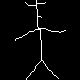
\includegraphics{80x80_thinning.png} 
	\caption{ Comparison of original image (left) and skeletonised one (right)}
\end{figure}
After small scale tests, newly-generated dataset speed up the training process, reducing one third of run-time.

\section{TensorFlow-related Tuning}
\subsection{Data Type}
The default data type (\texttt{tf.DType}) for numbers in tensors is \texttt{tf.float32} and for better memory performance, we decided to change it into \texttt{tf.bfloat16}, 16-bit truncated floating-point type, which makes both our neural network models even fit on mid-end computers with 7.7 GiB main memory with 1000 MiB swap, without affecting accuracy obviously (less than 1\% dropping rate).

\subsection{TFRecord}
Unlike other high-level deep learning API such as Keras\footnote{\url{https://keras.io/}}, TensorFlow does not implement HDF5 interface, a high-performance portable structured data format developed by HDF Group\footnote{\url{https://www.hdfgroup.org/}}, or supports it via h5py\footnote{\url{https://www.h5py.org/}}, though the possible alternative (tftables\footnote{\url{https://github.com/ghcollin/tftables}}) is available without official support. Instead, TensorFlow created its own pipeline-compatible API \texttt{tf.data} to create high-speed data structure \texttt{TFRecord}, to replace previous hard-to-use interface \texttt{QueueRunner}\cite[pp.~338]{geron2017hands} since 2017. Pre-processing data can be somewhat time-consuming, but once TFRecord files is an one-off solution of efficient training.

There are several ways to prepare data in TensorFlow, and the simplest one is preparing in Python language, using \texttt{tf.placeholder} as variable place holders and being fed into \texttt{feed\_dict} parameter. When in each step of training or testing, new batch of data come into models.

In practice, we try to use \texttt{Numpy} arrays directly. When all data is loaded into memory, dataset can be created by arrays. And after small scale experiments, we found that the method may copy the same block array contents for multiple times, which lessen loading speed in our case.

According to TensorFlow official API manual\footnote{\url{https://www.tensorflow.org/api\_guides/python/reading\_data}}, \texttt{feed\_dict} is the least efficient way to load data.
In TensorFlow, every independent data is regarded as an object in \texttt{tf.train.Example}, using \texttt{proto3} protocol to serialise data.
Here is the code snippet to create a TFRecord file by reading image contents and setting a unique label.
\begin{lstlisting}[language = Python, caption = TFRecord File Creation]
with open(FILENAME, "rb") as fp:
	image_data = fp.read()
	features = {
	"Images": _bytes_feature(image_data),
	"Labels": _int64_feature(label_index),
	}
	example = tf.train.Example(features =\
tf.train.Features(feature = features))
	tfrecord_writer.write(example.SerializeToString())
\end{lstlisting}
Where \texttt{\_bytes\_feature} and \texttt{\_int64\_feature} is helper functions to create a \texttt{Feature} object in TensorFlow.
And these data can be loaded into TensorFlow by simply \texttt{dataset = tf.data.TFRecordDataset(FILENAME)} and according to pipeline mechanism, speed improvement is dramatic. (In our case, data loading time is reduced from more than 50 seconds to 20 seconds.)

\subsection{Eager Execution}
Google TensorFlow development team released eager evaluation as experimental feature in 2017 and became formal after TensorFlow v1.7.0, which is ``an imperative, define-by-run interface'' to achieve faster debugging process more interactively and intuitively. Without building graphs as usual, basically it turns TensorFlow from declarative language to imperative one. Although we write this report, not all APIs support eager evaluation currently.

For most cases, user simply invoke \texttt{tf.enable\_eager\_execution()} at the beginning of TensorFlow-related code. And noticeably, eager evaluation works pretty good with \texttt{Numpy}. Although there are only a small of EE-specific APIs, most of current APIs are EE-compatible.
\begin{lstlisting}[language = Python, caption = Rewritten CNN Core Code Using Eager Eexecution]
EPOCHES = 1000
optimizer = tf.train.AdamOptimizer(learning_rate = 1e-3)
batch_size = 32
for step in range(EPOCHES):
	batch_data, batch_label = raw_data.train.next_batch(batch_size)
	batch_data = batch_data.reshape([-1 ,48, 48, 1])
	optimizer.minimize(lambda: loss(step, batch_data, batch_label))
\end{lstlisting}

\section{General Hyperparameter Adjustments}
In machine learning, a hyperparameter is a parameter whose value is set before the learning process begins. And there are some tricks that we learnt from other ones' code when we train our GANs, which may not be verified by traditional mathematical methods. However, in practice they work very well and we try to find evidences to back them.
\begin{itemize}
	\item According to \cite{Srivastava:2014:DSW:2627435.2670313}, we set our dropout rate to 50\%.
	\item ADAM optimiser is always our priority based on \cite{DBLP:journals/corr/SalimansGZCRC16}.
	\item At least in our CycleGAN training, we sometimes found that if we train discriminator more frequently, we can get a better result.
	\item Apply $ \tanh $ on the output of the last layer of the generator $ G $.
	\item In GAN-related papers, the loss function used to optimise $ G $ is always $ \min(\log{(1-D)}) $, but after reading several open-source code, people tend to use $ \max(\log{D}) $ practically. It is said that ``the first formulation has vanishing gradients early on''\cite{goodfellow2014generative}.
	\item After multiple experiments, we noticed that general performance of sampling from uniform distribution is much worse than sampling from Gaussian distribution. And the paper\cite{DBLP:journals/corr/White16a} seems to support our ideas in details.
	\item For Conditional GANs, use an embedding layer, and keep embedding dimensionality low and upsample to match image channel size.
	\item Also some suggests that label smoothing may be a good option to fast converge. Instead of giving a defined integer value (fake = 0 and real = 1), one can give a float-point number from 0.0 to 0.5 to stand for fake label and a number from 0.5 to 1.0 to stand for real one.  But in reality, we cannot apply that since it is really difficult to change code from \texttt{int32}-represented labels to \texttt{float32}-represented ones without any mistakes.
\end{itemize}